\documentclass[12pt]{article}
\usepackage{amsmath,amssymb,amsthm}
\usepackage{graphicx,mathabx}
\usepackage{xcolor}
\usepackage{tikz}
\usepackage{placeins}
\usepackage{lipsum}
\usepackage[shortlabels]{enumitem}
\usepackage{placeins}
\usepackage[makeroom]{cancel}
\usepackage{mathrsfs}
\newcommand\tab[1][1cm]{\hspace*{#1}}
\def\blankpage{%
      \clearpage%
      \thispagestyle{empty}%
      \addtocounter{page}{-1}%pdf
      \null%
      \clearpage}
\begin{document}
\title{TCSS 343 - Week 7}
\author{Jake McKenzie}
\maketitle
\noindent\centerline{\textbf{Graph Algorithms and some NP Completeness}}\\\\\\\\\\\\\\\\
\begin{center}
    ``Finding a needle in a haystack is actually quite easy. It's finding a very specific piece of hay in a haystack that happens to be hard." \\$\dots$\\ Avi Wigderson
\end{center}
\begin{center}
    ``People say nothing is impossible, but I do nothing every day'' \\$\dots$\\ Winnie-the-Pooh
\end{center}
\begin{center}
    ``It is not enough to be in the right place at the right time. You should also have an open mind at the right time." \\$\dots$\\ Paul Erd\H{o}s
\end{center}
\newpage
\noindent 0. Modify Kruskal's algorithm to find the maximum spanning tree.\\
\fbox{
    \parbox{10cm}{
      KRUSKAL \\
      
      $T = \emptyset$ \\
      FOR each vertex $v \in V$ {\sc Make-Set}($v$)
      
      Sort edges of $E$ in increasing order by weight \\
      FOR each edge $e=(u,v) \in E$ in order DO
      \begin{itemize}
      \item[] IF {\sc Find-Set}($u$) $\neq$ {\sc Find-Set}($v$) THEN
	\begin{itemize}
	\item[] $T = T \cup \{ e \}$
	\item[] {\sc Union-Set}($u,v$)
	\end{itemize}
      \end{itemize}
  }}
  \newpage
  1. Modify Prim's algorithm to find the maximum spanning tree.\\
  \fbox{
    \parbox{10cm}{
      PRIM(r)\\
      
      For each $v \in V$ DO
      \begin{itemize}
      \item[] {\sc Insert}($PQ,v,\infty$)
      \end{itemize}
	  {\sc Decrease-Key}$(PQ,r,0)$ \\
	  WHILE $PQ$ not empty DO
          \begin{itemize}
          \item[] $u$ = {\sc Deletemin}($PQ$)
	  \item [] (output edge $(u, visit(u))$ as part of MST)
          \item[] For each $(u,v) \in E$ DO
            \begin{itemize}
            \item[] IF $v \in PQ$ and $w(u,v) < $ key($v$) THEN
            \item[] ~~~~visit[$v$] = $u$
            \item[] ~~~~{\sc Decrease-Key}($PQ,v,w(u,v)$)
            \end{itemize}
          \end{itemize}
  }}
\newpage
\noindent 2. Give an example of a weighted connected undirected graph $G$ $=$ $(V,E)$ and a vertex $v$, such that the 
minimum spanning tree of $G$ is the same as the shortest-path tree at $v$.\\\\\\\\\\\\\\\\\\\\\\\\\\\\
3. Give an example of a weighted connected undirected graph $G$ $=$ $(V,E)$ and a vertex $v$, such that the 
minimum spanning tree of $G$ is very different from the shortest-path tree at $v$.\\\\\\\\\\\\\\\\\\\\\\\\\\\\
4. Can the two trees be completely disjoint?
\newpage
\noindent With this problem I want to present a 
problem to you and ask you why the greedy algorithm fails.\\\\
Imagine we have a wizard that knows a few spells. 
Each spell has 3 attributes: Damage, cooldown time, and a cast time. \\\\
\textbf{Cooldown time:} the amount of time (t) it takes 
before being able to cast that spell again. 
A spell goes on ``cooldown" the moment it begins casting.\\\\
\textbf{Cast time:} the amount of time (t) it takes 
to use a spell. While the wizard is casting 
something another spell cannot be cast and 
it cannot be canceled. \\\\
\textit{The question is:} \textbf{How would you maximize damage 
given different sets of spells?} \\\\
It is easy to calculate the highest damage per cast 
time. But what about in situations where it is better 
to wait then to get ``stuck" casting a low damage 
spell when a much higher one is available...for example consider
the two sets of spells:\\\\\\
Chill Touch: $100$ damage at a rate of $1$ second per cast with a $10$ second cooldown. \\\\
Mage Hand. $10$ damage at a rate of $4$ second per cast with a $0$ second cooldown.\\\\
Optimal spell ordering $\Sigma =\{$Chill Touch, Mage Hand, Wait, Repeat$\}$\\\\
5. Given an arbitary amount of time $t$ what is the maximum amount of spells
we can cast $S$?
\newpage
\noindent Now imagine that there is one spell, henceforth called the Eldritch Blast, 
which does a very, very large amount of damage, has $0$ casting time, and has 
some positive cooldown $n$. If all the other spells do much less damage than the 
Eldritch Blast, it will clearly be optimal to cast the Eldritch Blast every n seconds and 
then optimize the cooldown time with the weaker spells.\\\\
6. Why does the greedy algorithm work in this case?\\\\\\\\\\\\\\\\\\\\
Now, assume all the other spells also have cooldown $n$. 
If one optimizes a given n-second downtime with these spells, 
then the same spell-sequence will also be possible in the next 
$n$-second downtime, and so we can assume the solution is $n$-periodic.\\\\
7. Why does the greedy algorithm fail in this case?\\\\\\\\\\\\\\\\\\\\
8. Would you say this problem is NP-Complete? NP-Complete problems have the 
highest complexity of any problem in NP, which are the class of problems which can
be quickly checked to be true.
\newpage
\noindent For this problem and many problems, we can abstract out the details like we just did
and reduce the problem to it's key constituent parts. When you employ this
design technique you'll begin to notice that many problems you have reduce to problems
to classes of problems. This is the most powerful design technique I know of when it 
comes to algorithms.\\\\
9. Of the problems you've covered in class, which does this problem degenerate too? Describe for 
which cases this problems degrenates to that problem you've already covered.\\\\\\\\\\\\\\\\\\\\\\\\\\\\\\\\
A. Can you produce an informal algorithm that attempts to solve this problem?
\newpage
\centerline{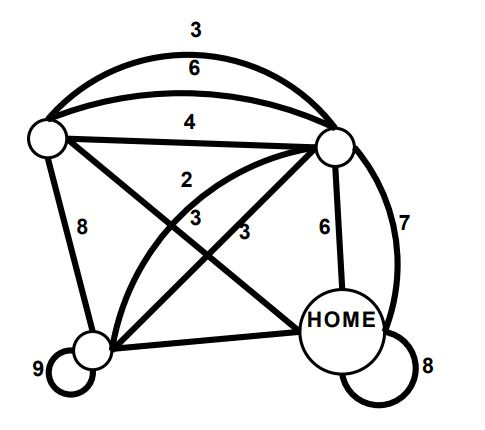
\includegraphics[scale = .45]{jogger.jpg}}
\noindent B. You're given a weighted, undirected graph $G$ with loops(edges that loop back on themselves), 
 multiple edges and only positive edge weights. There is a special node named ``Home" and you're given a positive integer $i \geq 0$.
 Can you find a path for the jogger $j$ that starts from home, travels the distance $i$ and returns home without repeating an edge while notes can be repeated?
\\\\We've talked previously in this packet about a problem that was disguised as a problem that we already knew. Reduce the jogger problem into the subset sum problem. 
 Since we can use jogger to solve subset sum the following must be true for the jogger algorithm $J$ and subset sum algorithm $SS$: \\
 \centerline{``cost of $SS$" $=$ ``times we use $J$" $\times$ ``cost of $J$" $+$ ``cost of the reduction"} \\
 \textbf{Remark:} This is how you show that a problem is NP-Complete, by showing that 
 your problem can be reduced to other problems in NP.
\newpage 
\noindent C. Prozve or disprove the following lemma: If each edge weight for a graph is increased by 1, then the minimum spanning tree does not change.\\\\\\\\\\\\\\\\\\\\\\\\\\\\\\\\\\\\
D. Prove or disprove the following lemma: If each edge weight for a graph is decreased by 1, then the minimum spanning tree does not change.
\newpage
\noindent F. Show that there's a unique minimum spanning tree (MST) in case the edges' weights are pairwise different ($w(e)$ $\neq$ $w(f)$ for $e$ $\neq$ $f$)\\\\
(\textbf{Hint: }If you employ Prim, Kruskal, or any of the other greedy minimum spanning tree algorithms, you can find that the weights needn't be added, only compared. 
What does this imply about collection of edge weights that make up each minimum spanning tree? What do we know about the weights of both graphs?)\\\\\\\\\\\\\\\\\\\\\\\\\\\\\\\\\\\\
\noindent 10. Assume that $G$ is a positive weighted graph. 
Under what condition does Prim's and Kruskal's algorithm on $G$  
yield the same minimum spanning trees? If they never do, explain why.
\newpage
\noindent For the next few problems state whether these desiderata are true or false and justify your work.\\\\
11. In an undirected graph, the shortest path between two nodes lies on some minimum spanning
tree.\\\\\\\\\\
12. If the edges in a graph have different weights, then the minimum spanning tree is unique.\\\\\\\\\\
13. Let $\Sigma$ be an algorithm that operates on a list of $n$ objects, 
where $n$ is a power of two. $\Sigma$ spends $\Theta(n^2)$ time dividing its input 
list into two equal pieces and selecting one of the two pieces. It 
then calls itself recursively on that list of $\frac{n}{2}$ elements. Then $\Sigma$'s 
running time on a list of n elements is $O(n)$.\\\\\\\\\\
14. Assume we deleted an edge from a graph $G$ which we will denote $G'$. The minimum spanning tree of $G'$ will 
have a number of edges no more than the number of edges of the minimum spanning tree for $G$.\\\\\\\\\\
15. Breadth first search forms a minimum spanning tree while depth first search does not.\\\\\\\\\\
16. The maximum number of minimum spanning trees is three for a positively weighted undirected graph.
\newpage
\noindent 17. The money game is as follows. Each vertex must give each vertex 1 to each neighboring 
vertex each turn or it can take 1 from each neighboring vertex. The aim of the game is to
get every node in the black (at least zero) in the fewest number of turns. Can you solve the money games 
for the following graphs? If you can't, can you find out why? \\\\
\textbf{HINT: } What's different about these two graphs?\\\\\\\\
\centerline{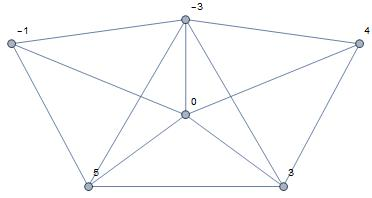
\includegraphics[scale = .8]{graph1.jpg}}\\\\
\centerline{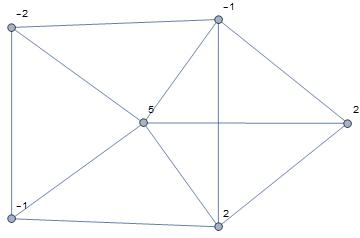
\includegraphics[scale = .8]{graph2.jpg}}
\newpage
\noindent 18. To solve the money game optimally is an open question in mathematics and computer science.
 This an open question, which means 
at least a few smart people have thought about it and failed to solve it, but that doesn't mean 
we can't think about it! A property that is known about the money game:
To have a solvable money game you must have enough money equal to the genus of a graph where 
the genus $=$ (number of Edges) $-$ (number of Vertices) $+$ $1$.\\\\
Design an algorithm that attempts to solve the money game in the least number of moves. 
\end{document}